%!TEX root = ../IfN-LaTex.tex
%!TEX spellcheck

%\label{chap:Main}
%
%\begin{itemize}
%\item Introduction/Motivation
%\item Basics/Literature survey
%\item Experimental set-up
%\item Test evaluation
%\item Summary and prospect
%\item Appendix
%\end{itemize}

%In this chapter ... At first, the general ... Afterwards, ... This chapter is mainly based on ... ...described in more detailsection{Basics}
\chapter{Basics}
\label{chap:Basics}
%In this chapter the algorithms, methods, ideas, programmes, etc. used in the thesis are explained. What were the premises of the thesis? How do others solve the problem? What is of further use, and what isn't? And why? In general, everything that was used for the thesis, and which wasn't of the author's origin, should be introduced here.
In this chapter, the foundations for the developed multi-source localization algorithm are laid. First, the signal model is introduced, and the basic assumptions, as well as the setup, are explained. Based on this, beamforming and the estimation of the closely related \ac{DOA} are discussed. Furthermore, the source classification using \acp{GMM} is introduced, as an important aspect of the developed classification algorithm. Finally, the state of the art of multi-source localization algorithms will be discussed and put in relation to each other.

\section{Signal Model}
\label{sec:signal_model}

In the beginning, the signal model has to be determined, which is the basis for the description of beamforming and acoustic localization. Considering a microphone array of $M$ microphones, positioned at $\vect{\breve{r}}_m = (\breve{r}_{m,x},\breve{r}_{m,y})^T$, receiving multiple signals over an acoustic channel from $Q$ sources at position $\vect {\oast r}_q = (\oast r_{q,x}, \oast r_{q,y})^T$ as illustrated in figure \ref{fig:sig_mode_doa}. In this thesis, an underscore is used to denote a column vector, and $^T$ is the transposed. The acoustic channel is formed by a superposition of the propagation on a direct path and a multitude of propagations on the indirect path, originating from the surrounding sources. \\
In figure \ref{fig:equiv_block} the equivalent block diagram for the signal arriving at microphone $m$ is shown which can mathematically be described as

\begin{equation}
x_m(n)=\sum^{Q}_{q=1}s_q(n) \ast h_{mq}(n) + v_m(n), \;  \forall \ m \in \{ 1,...,M\},
\label{eq:sig_model_time}
\end{equation}

where $x_m(n)$ represents the signal recorded by a microphone $m$, $s_q(n)$ represents the signal emitted by source $q$ and $h_{mq}(n)$ represents the room impulse response between the $q$'th source and the $m$'th microphone. They are connected by the convolution operator $\ast$. The microphones used are ideal and omnidirectional. Additionally, noise $v_m(n)$ is considered at any microphone $m$, which is uncorrelated across the microphone channels. For convenience, all signals are considered as time discrete signals, where $n$ denotes the discrete time index.\\


\begin{figure}[!t]
	\centering
	\begin{minipage}[t]{.45\textwidth}
		  \def\svgwidth{1\linewidth}
		  \small\input{figures/reverb.pdf_tex}
		\caption{Schematic diagram of sound propagation in a room from $Q$ sources to the microphone $m$}
		\label{fig:sig_mode_doa}
	\end{minipage}%
	\hfill
	\begin{minipage}[t]{.45\textwidth}
		\centering
		\begin{tikzpicture}

	\matrix (m1) [row sep=10mm, column sep=7mm]
	{
		\node[dspnodeopen]         		   	(m00) {$s_1(n)$};  		&
		\node[dspfilter,minimum width=1.4cm]	(m01) {$h_{mq}(n)$}; 	&
		\node[coordinate]                   (m02) {};          		&
		\node[coordinate]                   (m03) {};          		&
		\node[coordinate]                  	(m04) {};				&
		\node[coordinate]                  	(m05) {};				\\
		%--------------------------------------------------------------------
		\node                 				(m10) {$\cdots$};  &
		\node 			                  	(m11) {$\cdots$};  &
		\node[dspadder]                  	(m12) {};          &
		\node[dspnodeopen, dsp/label=above] (m13) {$v_m(n)$};  &
		\node[coordinate]                  	(m14) {};          \\
		%--------------------------------------------------------------------
		\node[dspnodeopen]         		   	(m20) {$s_Q(n)$};  		&
		\node[dspfilter,minimum width=1.4cm]	(m21) {$h_{mQ}(n)$}; 	&
		\node[dspadder]                    	(m22) {};          		&
		\node[dspadder]                    	(m23) {};          		&
		\node[dspmultiplier]			   	(m24) {};  %dsp/label=belo
		\draw [line width=0.25mm]
		([yshift=8pt]m24.west) -- ([yshift=-8pt]m24.west); 			&
		\node[dspnodeopen] 	     		 	(m25) {$x_m(n)$}; 		\\
		%--------------------------------------------------------------------
\\
		% \node[coordinate]                  (m11) {};          &
		% \node[dspmixer, dsp/label=right]   (m12) {$h[0]$};    &
		% \node[coordinate]                  (m13) {};          &
		% \node[dspmixer, dsp/label=right]   (m14) {$h[1]$};    &
		% \node[coordinate]                  (m15) {};          &
		% \node[dspmixer, dsp/label=right]   (m16) {$h[2]$};    &
		% \node[coordinate]                  (m17) {};          &
		% \node[dspmixer, dsp/label=right]   (m18) {$h[3]$};    &
		% \node[coordinate]                  (m19) {};          &
		% \node[coordinate]                  (m1X) {};          \\
		% %--------------------------------------------------------------------
		% \\
		% %--------------------------------------------------------------------
		% \node[coordinate]                  (m20) {};          &
		% \node[coordinate]                  (m21) {};          &
		% \node[coordinate]                  (m22) {};          &
		% \node[coordinate]                  (m23) {};          &
		% \node[dspadder]                    (m24) {};          &
		% \node[coordinate]                  (m25) {};          &
		% \node[dspadder]                    (m26) {};          &
		% \node[coordinate]                  (m27) {};          &
		% \node[dspadder]                    (m28) {};          &
		% \node[coordinate]                  (m29) {};          &
		% \node[dspnodeopen,dsp/label=above] (m2X) {$y(n)$};    \\
		% %--------------------------------------------------------------------
	};

	% \matrix (m1) [row sep=2.5mm, column sep=5mm]
	% {


	%--------------------------------------------------------------------

		%
		% \node[dspmultiplier,right=of c1,dsp/label=below] (c2) {}; &
		% \draw [line width=0.25mm] ([yshift=8pt]c2.west) -- ([yshift=-8pt]c2.west); &
		% \node[dspnodeopen,right= of c2] 	     		 (c3) {$y_m(n)$}; \\


	% };
	% \foreach \i [evaluate = \i as \j using int(\i+1)] in {0,1,...,4}
	% 	\draw[dspconn] (m2\i) -- (m2\j);
	% \foreach \i [evaluate = \i as \j using int(\i+1)] in {0,1}
	% 	\draw[dspconn] (m0\i) -- (m0\j);
	% 	\draw[dspconn] (m02) -- (m12);
	\draw[dspconn] (m00) -- (m01);
	\draw[dspconn] (m01) -| (m12);
	% \draw[dspconn] (m02) -- (m12);
	\draw[dspconn] (m11) -- (m12);
	\draw[dspconn] (m12) -- (m22);
	\draw[dspconn] (m13) -- (m23);
	\draw[dspconn] (m20) -- (m21);
	\draw[dspconn] (m21) -- (m22);
	\draw[dspconn] (m22) -- (m23);
	\draw[dspconn] (m23) -- (m24);
	\draw[dspconn] (m24) -- (m25);
\end{tikzpicture}


		\caption{Equivalent block diagram for one microphone}
		\label{fig:equiv_block}
	\end{minipage}
\end{figure}

\pagebreak

Equation \ref{eq:sig_model_time} may be brought from the time domain to the frequency domain by the Fourier transform:

\begin{equation}
X_m(\Omega)=\sum^{Q}_{q=1}S_q(\Omega) \cdot H_{mq}(\Omega) + V_m(\Omega), \; \forall \ m \in \{1,...,M\},
\label{eq:sig_model_freq}
\end{equation}

where $\Omega=2\pi f/f_s$ denotes the normalized frequency variable, where $f$ is the frequency and $f_s$ is the sampling rate. Here and in the following, capital letters are used to denote frequency domain variables. Equation \ref{eq:sig_model_freq} may also be written in a matrix representation
% $$\frac{1}{2}$$
% - free field model\\
% - far field\\

\begin{equation}
\begin{split}
  \begin{pmatrix} X_1 (\Omega) \\ \vdots \\ X_M(\Omega)\end{pmatrix}
  &=
  \begin{pmatrix}
  	{H}_{11}(\Omega)  & \ldots & {H}_{1Q}(\Omega) \\
  	\vdots   & \ddots & \vdots   \\
  	{H}_{M1}(\Omega)  & \ldots & {H}_{MQ}(\Omega)
  \end{pmatrix}
  \begin{pmatrix} S_1 (\Omega) \\ \vdots \\ S_Q(\Omega)\end{pmatrix}
  + \begin{pmatrix} V_1 (\Omega) \\ \vdots \\ V_M(\Omega)\end{pmatrix} \\[1em]
  \vect X(\Omega)&= \mat H(\Omega) \vect S(\Omega)+ \vect V(\Omega),\\
  \label{eq:sig_model_mat}
\end{split}
\end{equation}

% Simplification: dominance of the direct path\\

% \begin{equation}
% H_{mq}(\Omega) = |H'_{mq}(\Omega)|e^{-j\Omega f_s \tau_{mq}(\mat r_q)}+H''_{m,q}(\Omega)
% \end{equation}
% \begin{equation}
% H_{mq}(\Omega) \approx |H'_{mq}(\Omega)|e^{-j\Omega f_s \tau_{mq}(\mat r_q)}
% \end{equation}
where bold letters are used for matrices. \\
Since the absolute acoustic transfer functions $H_{mq}(\Omega)$ can only be identified up to a filtering, a reference point $r_0$ is introduced. Typically one microphone is chosen as a reference microphone, whose transfer function $H_{Rq}(\Omega)$ is related to the source spectrum $S_q(\Omega)$.

This turns the matrix $\mat H(\Omega)$ into the matrix of \emph{relative} transfer functions $\mat A(\Omega)$:
% When factoring out the introduced transfer function in \ref{eq:sig_model_mat}, equation \ref{eq:sig_model_relativ} is obtained

% \begin{equation}
% X_m(\Omega) = \frac{|H'_{mq}(\Omega)|}{|H'_{0q}(\Omega)|} e^{-j\Omega f_s (\tau_{mq}-\tau_{Rq})}S_q(\Omega)|H'_{0q}(\Omega)|e^{-j\Omega f_s \tau_{Rq}}+
% \end{equation}

\begin{equation}
\begin{split}
  \begin{pmatrix} X_1 (\Omega) \\ \vdots \\ X_M(\Omega)\end{pmatrix}
  &=
  \begin{pmatrix}
  	\frac{{H}_{11}(\Omega)}{H_{R1}(\Omega)}  & \ldots & \frac{{H}_{1Q}(\Omega)}{H_{RQ}(\Omega)} \\
  	\vdots   & \ddots & \vdots   \\
  	\frac{{H}_{M1}(\Omega)}{H_{R1}(\Omega)}  & \ldots & \frac{{H}_{MQ}(\Omega)}{H_{RQ}(\Omega)}
  \end{pmatrix}
  \begin{pmatrix} S_1 (\Omega) H_{R1}(\Omega) \\ \vdots \\ S_Q(\Omega)H_{RQ}(\Omega)\end{pmatrix}
  + \begin{pmatrix} V_1 (\Omega) \\ \vdots \\ V_M(\Omega)\end{pmatrix} \\[1em]
  \vect X(\Omega) &= \mat A(\Omega)  \vect S'(\Omega) + \vect V(\Omega),
  \end{split}
  \label{eq:sig_model_relativ}
\end{equation}

% \begin{equation}
% X(\Omega) = \frac{H(\Omega)}{H_{Rq}(\Omega)} \underbrace{S_q(\Omega)H_{Rq}(\Omega)}_{S'(\Omega)}+\underbrace{V(\Omega)H_{Rq}(\Omega)}_{V'(\Omega)}.
% \label{eq:sig_model_relativ}
% \end{equation}
where $\mat A(\Omega)$ is the transfer function matrix in regards to the reference point. Each column of matrix $\mat A(\Omega)$ can be called propagation vector $\vect A_q(\Omega)$ for source $q$: $\mat A_q(\Omega):=(\vect A_1(\Omega),...,\vect A_Q(\Omega))$. The transfer functions between the microphones and the reference point multiplied with the source signal is denoted as $\vect S'(\Omega)$. When dividing the elements of $\mat A(\Omega)$ in \ref{eq:sig_model_relativ} into magnitude and phase, the \ac{TDOA} becomes visible

\begin{equation}
A_{mq}(\Omega)= \frac{H_{mq}(\Omega)}{H_{Rq}(\Omega)} = \frac{|H_{mq}(\Omega)|}{|H_{Rq}(\Omega)|} e^{-j\Omega f_s (\tau_{mq}-\tau_{Rq})}.
\label{eq:relative_IR}
\end{equation}

The difference between the time delays of a microphone position and the reference point $\Delta\tau_{mq} = \tau_{mq}-\tau_{Rq}$ represents the relative time delay or \ac{TDOA}. \cite[Chapter~2]{madhu2010acoustic}\\
Due to the unknown position of the acoustic source, the absolute time delays $\tau_{mq}$ and $\tau_{Rq}$ cannot be obtained.
% The difference $\Delta\tau_{mq}$, however can be observed from \ref{eq:relative_IR}.
The difference, however, can be observed from \ref{eq:sig_model_relativ}.
To later obtain the angle $\varphi$, which is the \ac{DOA}, a model for the \ac{TDOA} and the transfer matrix $\mat A(\Omega)$, respectively, is needed. Therefore the array geometry and the position of the reference point $r_0$ has to be known. Furthermore, some constraints are needed. Far-field is assumed, which means that the distance between sources and microphones is much greater than the distance between the different microphones $\|\vect {\oast r}_q-\vect {\breve r}_m\| \gg \|\vect {\breve r}_{i}-\vect {\breve r}_{j}\|,\ \forall\ i,j \in \{1, ... M\ |\ i \neq j\}$. In this case, the signal propagation can be assumed as a plane wave. Moreover, free field model is assumed which means that anechoic conditions or no reflections are considered. \cite[Chapter~2]{madhu2010acoustic}
\begin{figure}[!ht]
	\subfloat[ULA\label{fig:ula}]{%
		  \def\svgwidth{.45\linewidth}
		  \small\input{figures/ula.pdf_tex}
	}
	\hfill
	\subfloat[UCA+C\label{fig:uca_c}]{%
		  \def\svgwidth{.45\linewidth}
		  \small\input{figures/uca2.pdf_tex}
	}
	\caption{Outline of different array geometries, to calculate the \acl{TDOA} . The red line is the difference of distance the sound coming from direction $\varphi_q$ has to travel between microphone $m$ and the reference point.}
	\label{fig:DOA}
\end{figure}
In general, this time delay can be stated with the help of the vectors from the reference point to the microphone positions $\vect r_{Rm} = \vect {\breve r}_m - \vect r_0$ as

\begin{equation}
\begin{split}
\Delta\vect{\tau}(\varphi_q)=\Bigg(\ & \frac{r_{R1,x}\cos(\varphi_q)+r_{R1,y}\sin(\varphi_q)}{c},\ \ \cdots, \\ & \frac{r_{RM,x}\cos(\varphi_q)+r_{RM,y}\sin(\varphi_q)\ }{c}\Bigg)^T,\\
\end{split}
\label{eq:timedelay}
\end{equation}

where $c$ is the speed of sound. To illustrate equation \ref{eq:timedelay}, two fundamental array geometries are considered. First, the \ac{ULA} geometry as shown in figure \ref{fig:ula} is used with a reference point $\vect r_0$ set to the first microphone. When utilizing this array in \ref{eq:timedelay} the following is obtained for the \ac{TDOA}:

\begin{equation}
\Delta\vect{\tau}_{\text{ULA}}(\varphi_q)=\Big(\ 0,\ \ \frac{r_{R2,x}\cos\varphi_q}{c},\ \cdots\ ,\ \frac{r_{RM,x}\cos\varphi_q}{c}\Big)^T,
\label{eq:ula}
\end{equation}

where $\varphi_q$ is the \ac{DOA} of source $q$ in the azimuth plane and $c$ is the speed of sound.\\
Another important geometry is the \ac{UCA+C} geometry seen in figure \ref{fig:uca_c}. The reference point $\vect r_0$ is commonly set into the center which results in

\begin{equation}
\begin{split}
\Delta\vect{\tau}_{\text{UCA+C}}(\varphi_q)=\Bigg(\ 0, \ \ & \frac{r_{R2,x}\cos\varphi_q+r_{R2,y}\sin\varphi_q}{c},\ \ \cdots ,\\ & \frac{r_{RM,x}\cos\varphi_q+r_{RM,y}\sin\varphi_q}{c}\ \Bigg)^T,\\
\end{split}
\label{eq:uca_c}
\end{equation}


as the \ac{TDOA} for an \ac{UCA+C}. As stated in chapter \ref{chap:introduction} only a \ac{UCA+C} with a radius of \SI{42}{\milli \metre} is considered in this work. When using the free field model and the further constraints for the \ac{TDOA} calculation in the propagation vector following is obtained

\begin{equation}
\vect A_q^{\text{ff}}(\Omega) = \exp\big(-j\Omega f_s \Delta\vect \tau(\varphi_q)\big),
\label{eq:transfer_free_field}
\end{equation}

where $A_q^{\text{ff}}(\Omega)$ is the propagation vector function for a source $q$ in the free field model.

\subsection{Spatial Covariance}
\label{subsec:spatial_cov}
Another important signal property is the covariance that describes the interdependencies between the microphone signals $\vect X(\Omega)$. To obtain this covariance, it is presumed that the signals are stochastic. When only considering one source ($Q=1$),
% , the source signals at the reference point collapse to a scalar $S'(\Omega)$ and
the spatial covariance matrix can be denoted as

% expectation value $E\{\cdot\}$ of microphone signals squared can be noted as
% where $\mat \Phi_{xx}(\Omega)$ denotes the Spatial covariance matrix of the signal at the microphones $X(\Omega)$. As a clarification, the matrix consists of the time delays of the desired signal between microphone pairs in an ideal environment as described at the end of section \ref{sec:signal_model}.

\begin{equation}
\begin{split}
\mat \Phi_{xx}(\Omega) &= \text{E}\{\vect X(\Omega)\vect X^H(\Omega)\} \\
 &= \vect A(\Omega) \text{E} \{ S'(\Omega)  S'^*(\Omega)\}\vect A^H(\Omega) + \text{E}\{\vect V(\Omega)\vect V^H(\Omega)\}\\
 &= \mat \Phi_{ss}(\Omega) + \mat \Phi_{vv}(\Omega),
\end{split}
\end{equation}

where $E\{\cdot\}$ represents the expectation value operator, $^*$ denotes the complex conjugate operator, $\mat \Phi_{ss}(\Omega)$ represents the source correlation matrix, $\mat \Phi_{vv}(\Omega)$ the noise correlation matrix and $(\cdot)^H$ the Hermitean operator. For uncorrelated source signals $S_q(\Omega)$ and $Q>1$ the spatial covariance is obtained as:

\begin{equation}
 \mat \Phi_{xx}(\Omega) = \sum_{q=1}^Q \mat \Phi^q_{ss}(\Omega) + \mat \Phi_{vv}(\Omega),
\end{equation}

where $\mat \Phi^q_{ss}(\Omega)$ is the covariance matrix of the $q$'th source signal. It is evident that the covariance matrix $\mat \Phi_{xx}(\Omega)$ is a superposition of the $Q$ source covariance matrices $\mat \Phi^q_{ss}(\Omega)$ and the noise covariance matrix $\mat \Phi_{vv}(\Omega)$.

\section{Beamforming}
\label{sec:beamforming}
Beamforming or spatial filtering is an array processing technique used to improve the quality of the desired signal in the presence of noise. This filtering is accomplished by a linear combination of the recorded signals $X_m(\Omega)$ and the beamformer weights $W_m(\Omega)$. In other words, the filtered microphone signals are summed together (compare with figure \ref{fig:filtersum}). When the filter weights are configured correctly, the desired signal is superimposed constructively.
\begin{figure}[ht]
	\centering
	\begin{tikzpicture}
	[
  	coordinate/.style={minimum height=1em,},
	]

	\matrix (m1) [row sep=2mm, column sep=20mm]
	{
		\node[dspmultiplier]			   	(m00) {};  %dsp/label=belo
		\draw [line width=0.25mm] 
		([yshift=8pt]m00.west) -- ([yshift=-8pt]m00.west); 			&
		\node[dspfilter, minimum width=20mm]					(m01) {$W_{1}(\Omega)$}; 	&
		\node[coordinate]                   (m02) {};          		&
		\node[coordinate]                   (m03) {};          		\\
		%--------------------------------------------------------------------
		\node[dspmultiplier]			   	(m10) {};  %dsp/label=belo
		\draw [line width=0.25mm] 
		([yshift=8pt]m10.west) -- ([yshift=-8pt]m10.west); 			&
		\node[dspfilter, minimum width=20mm]					(m11) {$W_{2}(\Omega)$};	&
		\node[coordinate]                   (m12) {};          		&
		\node[coordinate]                   (m13) {};          		\\

		% %--------------------------------------------------------------------
		\node[coordinate]                   (m20) {}; 				&
		\node[coordinate]                   (m21) {}; 				&
		\node[dspadder]                   	(m22) {}; 				&
		\node[dspnodeopen] 	     		 	(m23) {$Y(\Omega)$}; 		\\

		% %--------------------------------------------------------------------
		\node[dspmultiplier]			   	(m30) {};  %dsp/label=belo
		\draw [line width=0.25mm] 
		([yshift=8pt]m30.west) -- ([yshift=-8pt]m30.west); 			&
		\node[dspfilter, minimum width=20mm]					(m31) {$W_{M-1}(\Omega)$}; 	&
		\node[coordinate]                   (m32) {};          		&
		\node[coordinate]                   (m33) {};          		\\
		% %--------------------------------------------------------------------
		\node[dspmultiplier]			   	(m40) {};  %dsp/label=belo
		\draw [line width=0.25mm] 
		([yshift=8pt]m40.west) -- ([yshift=-8pt]m40.west); 			&
		\node[dspfilter, minimum width=20mm]					(m41) {$W_{M}(\Omega)$}; 	&
		\node[coordinate]                   (m42) {};          		&
		\node[coordinate]                   (m43) {};          		\\
		\\
	};
	\draw[dspflow] (m00) -- node [above]  {$X_1(\Omega)$} (m01);
	\draw[dspconn] (m01.east) -- (m22);
	\draw[dspflow] (m10) -- node [above]  {$X_2(\Omega)$} (m11);
	\draw[dspconn] (m11.east) -- (m22);
	% \draw[dspconn] (m20) -- (m21);
	% \draw[dspconn] (m21.east) -- (m22);
	\draw[dspconn] (m22) --   (m23);
	\draw[dspflow] (m30) -- node [above]  {$X_{M-1}(\Omega)$}(m31);
	\draw[dspconn] (m31.east) -- (m22);
	\draw[dspflow] (m40) -- node [above]  {$X_{M}(\Omega)$}(m41);
	\draw[dspconn] (m41.east) -- (m22);
\end{tikzpicture}
	\caption{Filter and sum beamformer.	Microphone signals \vect{X}$(\Omega)$ are multiplied with the beamformer weights \vect{W}$(\Omega)$ and then accumulated to the beamformer output signal $Y(\Omega)$.}
	\label{fig:filtersum}
\end{figure}

\pagebreak

In vector notation, the beamformer output signal can be written as

\begin{equation}
Y(\Omega) = \vect W^H(\Omega)\ \vect X (\Omega),
\label{eq:filter_sum}
\end{equation}

where $\vect X(\Omega)$ is defined in \ref{eq:sig_model_relativ} as vector of microphone spectra, $\vect W(\Omega)$ represents the vector of beamformer filter weights and $Y(\Omega)$ is the output signal of the beamformer. $(\cdot)^H$ is the hermitian (self-adjoint) operator. This beamformer weighting vector $\vect W(\Omega)$ may be determined, by solving a constrained optimization problem. These constraints are using the power $\phi_{yy}(\Omega)$ of $Y(\Omega)$ which can be written as,

\begin{equation}
\begin{split}
\phi_{yy}(\Omega) &= E\{Y(\Omega)Y^*(\Omega)\} \\
&= E\{\vect W^H(\Omega) \vect X(\Omega) \vect X^H(\Omega) \vect W(\Omega)\}\\
&= \vect W^H(\Omega) \mat \Phi_{xx}(\Omega)\vect W(\Omega).
\label{eq:bf_power}
\end{split}
\end{equation}
A very prominent approach to determine $\vect W(\Omega)$ is to minimize its output power $\phi_{yy}(\Omega)$ without distorting the desired signals. In the following, this beamforming approach is discussed in more detail.


% \begin{equation}
% P(\mat w) = \frac{1}{N}\sum^N_{t=1} |y(t)|^2 = \frac{1}{N}\sum^N_{t=1} \mat w^H \mat x(t)\mat x^H(t)\mat w  = \mat w^H \mat{\hat{\Phi}}_{xx}  \mat w
% \end{equation}

% \subsection{Generalized Cross-correlation}

% \begin{figure}[!ht]
% 	\centering
% 	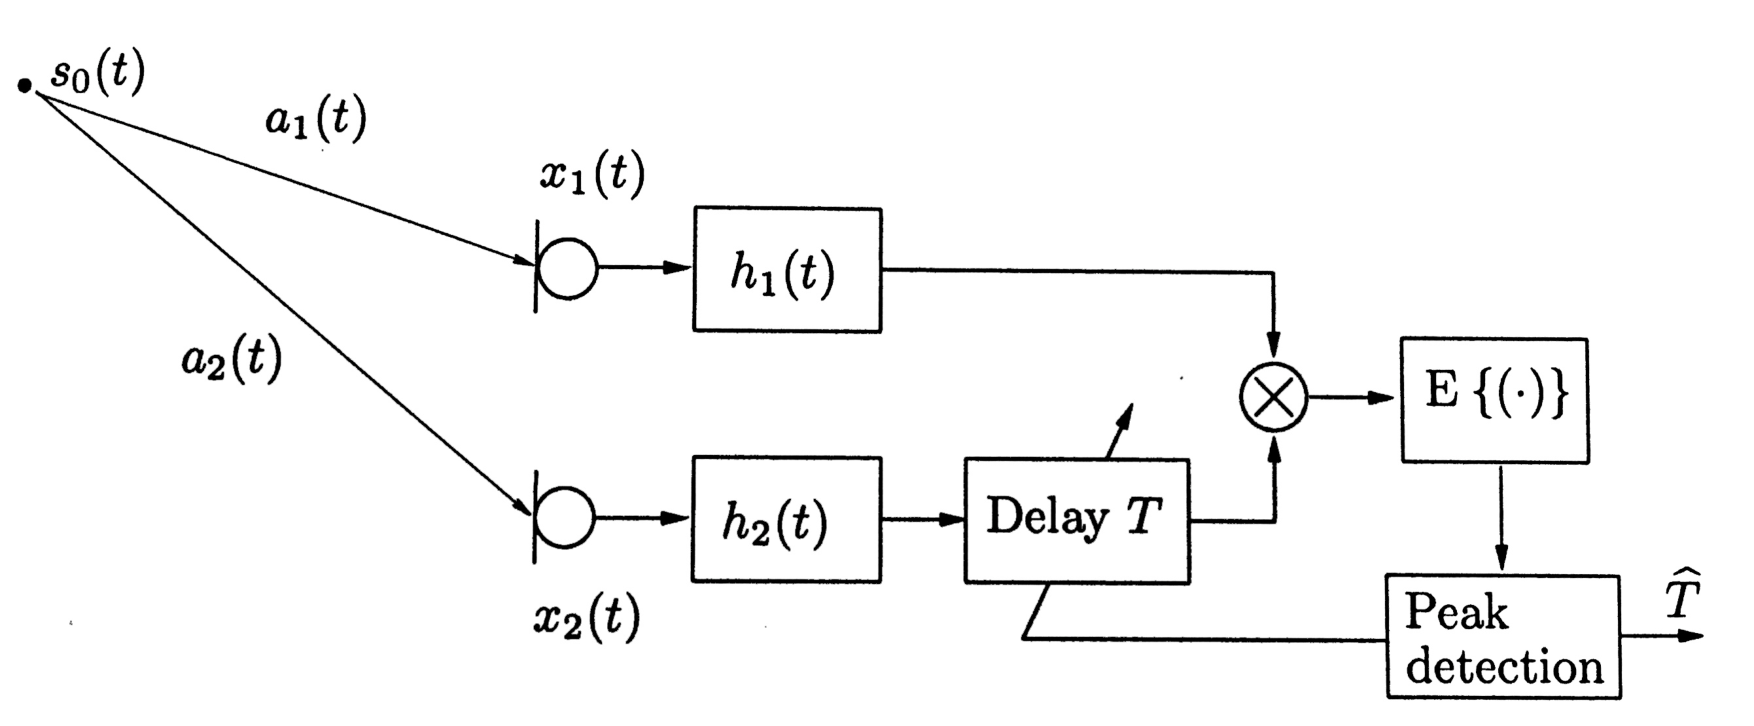
\includegraphics[width=0.80\textwidth]{figures/gcc.pdf}
% 	\caption{GCC}
% 	\label{fig:gcc}
% \end{figure}

\subsection{Minimum Variance Distortionless Response Filter}
\label{subsec:mvdr}
The \ac{MVDR} optimization criterion states that the output variance in equation \ref{eq:bf_power} shall be minimized, under the constraint of no distortion in steering direction $\theta$. This optimization can mathematically be described as

\begin{equation}
\begin{split}
\vect W^H(\Omega) \mat \Phi_{xx}(\Omega)\vect W(\Omega) \rightarrow \min_{\vect W(\Omega)} \\
\text{subject to } \vect W^H(\Omega) \vect D(\Omega,\theta) = 1,
\end{split}
\end{equation}

% \todo{Do I have to refer to \ref{fig:ula} or \ref{eq:realtive_IR}?}
% where $\phi_{yy}$ represents the power of \ref{eq:bf_power}, also stated as variance, at the output of the beamformer.
where $\vect D(\Omega,\theta)$ is the steering vector, which is calculated similarly to the modeled propagation vector $\vect A_q^\text{ff}(\Omega)$ and uses the \ac{TDOA} from equation \ref{eq:timedelay}: $\vect D(\Omega,\theta) = \exp(-j\Omega f_s \Delta \vect \tau(\theta))$. However, it represents the steering direction $\theta$ of the array and not the propagation direction $\varphi$ also called \ac{DOA} of the signal $S_q(\Omega)$. For convenience, the normalized frequency $\Omega$ is neglected but will be reintroduced when it is needed. The optimization may be solved using the technique of Lagrange multipliers \cite[Section~2,~Chapter~4]{lagrange}\cite[Chapter~6.2.5.6]{bronstein}, which results in
% \cite[Appendix~E]{bishop2016pattern}
\begin{equation}
\vect W_\text{CAP}(\theta) = \frac{\mat{\Phi}_{xx}^{-1} \vect D(\theta) } { \vect D^H(\theta) \mat{\Phi}_{xx}^{-1} \vect D(\theta) }.
\label{eq:w_capon}
\end{equation}

This beamforming technique is also known as Capon beamformer by the name of its inventor.
\cite{Capon1969,krim1996two}

%\todo{MVDR mit phiVV hier formulieren auf unterschiede hinweisen}

\subsection{Delay and Sum Beamformer}
\label{subsec:DS}
The \ac{DS} beamformer is a special case of the \ac{MVDR} beamformer.
The beamformer is optimized for the uncorrelated sound field as noise.
To derive the \ac{DS} beamformer, the optimization criterion has to be changed from minimizing the output power $\phi_{yy}$ to minimizing the noise after the beamformer weights $\vect W^H\mat \Phi_{vv}\vect W$.
%This is viable if the steering vector $D(\theta)$ is equal to propagation vector $\vect A_q(\phi)$. The derivation for this can be comprehended in the appendix (XXX). Employing this constraint the desired signal remains untouched in any case, which makes the beamformer more robust against deviation of the steering angle $\theta$ concerning the actual \ac{DOA}.
The resulting weight vector changes from \ref{eq:w_capon} to \footnote{Note that equation \ref{eq:w_capon} and \ref{eq:w_capon_mod} are equal only if $\vect D(\theta) = \vect A_q(\varphi)$. If the assumed steering vector $\vect D(\theta) \neq \vect A_q(\varphi)$, which is usually the case in realistic acoustic environments, equation \ref{eq:w_capon} will lead to signal distortions. Equation \ref{eq:w_capon_mod} on the other hand is more robust to steering vector mismatch as only the noise is minimized.}

\begin{equation}
\vect W(\theta) = \frac{\mat{\Phi}_{vv}^{-1} \vect D(\theta) } { \vect D^H(\theta) \mat{\Phi}_{vv}^{-1} \vect D(\theta) }. \label{eq:w_capon_mod}
\end{equation}

Assuming a spatial uncorrelated noise field, the noise power $\mat \Phi_{vv}$ reduces to a unit matrix $\mat \Phi_{vv} \rightarrow \phi_{vv} \mat I$. With this assumption used in \ref{eq:w_capon_mod}, the \ac{DS} weights can be stated as

\begin{equation}
\begin{split}
\vect W_\text{DS}(\theta) &= \frac{\phi_{vv} \vect D(\theta) } {\phi_{vv} \vect D^H(\theta)\vect D(\theta)  }\\
&= \frac{\vect D(\theta)}{M}. \label{eq:w_ds}
\end{split}
\end{equation}

The number of microphones $M$ is seen in the denominator because squaring reduces the steering vector, which consists of $M$ unit vectors to the number of elements. This beamformer can be seen as time compensation before the summation. Therefore the name \emph{delay \& sum} beamformer is used. \cite[Chapter~2]{brandstein2013microphone}

\section{Acoustic Speaker Localization}
\label{sec:localization}
% Direction-of-Arrival Estimation
The \ac{ASL} techniques known from literature can broadly be divided into two parts. On the one hand the parametric approach exists. Here a multidimensional search has to be deployed to find all estimates at once. One of the most frequently used parametric approaches is the \ac{ML} technique. On the other hand there are the spectral-based algorithms, which are computationally more feasible than the preceding one, but may suffer from inaccuracy. In this approach, a spectrum-like function is formed, which can be searched for the parameters of interest. Spectral-based methods can again be subdivided into beamforming and subspace-based techniques. One of the most popular subspace-based techniques is \ac{MUSIC}, which utilizes an eigenvalue decomposition, that again is computationally very complicated. Subspace-based techniques is a field of great research interests with the development of multiple techniques like CSSM \cite{1164667}, TOPS \cite{yoon2006tops}, FRIDA \cite{pan2017frida} or WAVES \cite{di2001waves}. In this work, the beamforming technique is used and will be discussed in more detail. \cite{krim1996two}

% - Spectra-based\\
% Subspace-based
\subsection{Steered Response Power}
\label{subsec:SRP}
The \ac{SRP} method tries to estimate the \ac{DOA} by steering a beamformer towards a set of possible directions and calculating the resulting power. In a second step, the angle that maximizes the power is chosen as the \ac{DOA} estimate. This method can be applied with different kinds of beamformers. \\
The output power of the Capon beamformer can be written by inserting \ref{eq:w_capon} in \ref{eq:bf_power} as

\begin{equation}
\begin{split}
P_\text{CAP}(\Omega,\theta) &= \vect W_\text{CAP}^H(\Omega, \theta) \mat \Phi_{xx}(\Omega)\vect W_\text{CAP}(\Omega, \theta)\\
&=
\frac{\vect D(\Omega, \theta)^H \mat{\Phi}_{xx}^{-1}(\Omega)  } { \vect D^H(\Omega, \theta) \mat{\Phi}_{xx}^{-1}(\Omega) \vect D(\Omega, \theta) }
\mat \Phi_{xx}(\Omega)
\frac{\mat{\Phi}_{xx}^{-1}(\Omega) \vect D(\Omega, \theta) } { \vect D^H(\Omega, \theta) \mat{\Phi}_{xx}^{-1}(\Omega) \vect D(\Omega, \theta) }\\
&=...\\
&=
\frac{1}{\vect D^H(\Omega, \theta)\ \mat{\Phi}_{xx}^{-1}(\Omega)\ \vect D(\Omega, \theta)}.
\end{split}
\label{eq:p_capon}
\end{equation}

% Here, the \ac{STFT} notation stated in \ref{} is reintroduced.
Respectively, when using \ref{eq:w_ds} in \ref{eq:bf_power}, the power output of the \ac{DS} beamformer can be stated as

\begin{equation}
P_\text{DS}(\Omega,\theta) = \frac{\vect D^H(\Omega, \theta)\ \mat{\Phi_{xx}}(\Omega)\ \vect D(\Omega, \theta)}{M^2}.
\label{eq:p_ds}
\end{equation}

% The results are also called spatial power spectrum because they are dependent on the frequency $\Omega$ and the steering direction $\theta$.\\
In the next step, the angle for the maximum steered power has to be found. This
can be done in two ways. The broadband method takes the mean over all frequencies and searches for the maximum afterwards. In the frequency \ac{DOA} estimation, the averaging over frequencies is dropped, and the maximum search is done  in every frequency.
% Before noting the mathematical equation for the broadband approach, the \ac{SRP-PHAT} shall be introduced. More robust localization were accomplished, when using the \emph{coherence} matrix instead of the covariance matrix. This change is done because the absolute power in every bin varies allot. The approach is, to normalize the covariance matrix by canceling out the absolute power and thus only the phase is holding all information, which is mathematically noted as
% \begin{equation}
% J_{xx}^{ij}(\Omega) = \frac{\phi_{ij}(\Omega)}{\sqrt{\phi_{ii}(\Omega)\phi_{jj}(\Omega)}},\; \forall i,j \in \{1,...,M\}
% \label{eq:coherence}
% \end{equation}
% where $J_{xx}^{ij}(\Omega)$ are the entries of the $M \times M$ coherence matrix $\mat J_{xx}$ and $\phi_{ij}$ are the elements of the covariance matrix $\mat \Phi_{xx}(\Omega)$. \\
% When using the coherence $\mat J_{xx}(\Omega)$ from \ref{eq:coherence} instead of the covariance $\mat \Phi_{xx}(\Omega)$ in \ref{eq:p_capon} and \ref{eq:p_ds} we obtain
% \begin{equation}
% P_\text{CAP,PHAT}(\Omega, \theta) = \frac{1}{\vect D^H(\Omega, \theta)\ \mat{J}_{xx}^{-1}(\Omega)\ \vect D(\Omega, \theta)},
% \label{eq:p_capon_phat}
% \end{equation}
% and
% \begin{equation}
% P_\text{DS,PHAT}(\Omega, \theta) = \frac{\vect D^H(\Omega, \theta)\ \mat{J}_{xx}(\Omega)\ \vect D(\Omega, \theta)}{M^2}.
% \label{eq:p_ds_phat}
% \end{equation}
The broadband method can be stated as following:
% By averaging the power over frequencies $\overline{P}^\text{b}(\theta)$,  and taking the $\arg \max$, the \ac{DOA} as a broadband estimate is finally obtained

% - SRP-PHAT DS\\
% - SRP-PHAT Capon\\
% %\subsection{Multi-source DOA}
% Broadband\\

\begin{equation}
\begin{split}
\hat{\varphi} &= \arg \max_{\theta}\frac{1}{2\pi}\int^\pi_{-\pi}P(\Omega,\theta)\mathrm{d}\Omega\\
 &= \arg \max_{\theta} \overline{P}^\text{b}(\theta).
\end{split}
\label{eq:doa_est_broadband}
\end{equation}

When averaging across frequencies is neglected, it yields a \ac{DOA} estimate for every frequency, which is noted as

\begin{equation}
\hat{\varphi}(\Omega) = \arg\max_{\theta}P(\Omega,\theta).
\label{eq:doa_est_freq}
\end{equation}

Receiving one value per frequency may enable a real multi-source detection, under the assumption, that the sources are spectrally disjoint. Broadband and frequency SRP values are distinguished by the dependence on frequency $\Omega$.
The broadband \ac{SRP} may also be weighted before mean taking. This can be done in different ways. One of them is the \ac{PHAT}. Mathematically this can be stated as

\begin{equation}
\begin{split}
\hat{\varphi} &= \arg \max_{\theta}\frac{1}{2\pi}\int^\pi_{-\pi}\frac{1}{\phi_{xx}(\Omega)}P(\Omega,\theta)\mathrm{d}\Omega\\
 &= \arg \max_{\theta} \overline{P}^\text{b}_\text{PHAT}(\theta).
\end{split}
\label{eq:doa_est_broadband_phat}
\end{equation}
The \ac{PHAT} weighted steered mean power is stated as $ \overline{P}^\text{b}_\text{PHAT}(\theta)$. It is assumed that the sound field is homogeneous, which means that the microphones have the same amount of variance $\phi_{xx}(\Omega)$.\footnote{Note that the variance $\phi_{xx}$ are the values on the main diagonal of the covariance matrix} Furthermore, the assumption decreases the computational load.
% \begin{equation}
% \begin{split}
% \phi_{ii} &= \phi_{jj}, \; \forall \ i,j \in \{ 1...M| i \neq j\}\\
%  &= \phi_{xx},
% \end{split}
% \label{eq:assumtion_homogen}
% \end{equation}
% where $\phi_{ii}$ and $\phi_{jj}$ are the values on the main diagonal of the covariance matrix.
This weighting leads to canceling out the absolute power. Thus only the phase is holding all information, and all spectral parts are having equal share in the broadband \ac{SRP} in respect to the mean. \cite[Chapter~8]{brandstein2013microphone}\cite{madhu2008scalable}\\

% \begin{figure}[!ht]
% 	\centering
% 	\includegraphics[width=0.45\textwidth]{figures/SPS_compare.png}
% 	\caption{Comparison}
% 	\label{fig:comparision}
% \end{figure}

\subsection{Theoretical Steered Power Spectrum and Aliasing}


The theoretical Steered Power Spectrum can be used to evaluate different types of beamformers. They are calculating the response of a microphone array to a wavefront with a certain \ac{DOA} for all parameters. As stated in chapter \ref{chap:introduction} in this work only the azimuth-plane is considered. So the response is dependent on the azimuth angle $\theta$ and the normed frequency $\Omega$. The theoretical steered power spectrum can be calculated, when considering a signal as in \ref{eq:sig_model_relativ} but with neglecting the noise $\vect V(\Omega) = 0$ and setting the modified source signal $S'(\Omega) = 1$ which can be seen as a white noise signal. %The response is then obtained when calculating the output power of the beamformer in decibel:
In dB, the \ac{SRP} then reads\footnote{Note that this is very similar to the well known beampattern. Here (equation \ref{eq:p_theory}), the beamformer weights are changed as apposed to changing $\vect A(\Omega)$ depending on $\theta$.}:

\begin{equation}
P_\text{theory}(\Omega,\theta) \mid _\text{db} = -10\log_{10}(|\vect W^H(\Omega,\theta)\vect A(\Omega)|^2).
\label{eq:p_theory}
\end{equation}

Different beamformer weight vectors $\vect W(\Omega,\theta)$ can be compared, for instance those of \ac{DS} beamformer \ref{eq:w_ds} or Capon beamformer \ref{eq:w_capon}. Steering vector $\vect D(\Omega,\theta)$ and propagation vector $\vect A(\Omega)$ are dependent on the array geometry and can for example be calculated with \ref{eq:ula} and \ref{eq:uca_c} in \ref{eq:transfer_free_field}. \cite[Chapter~2]{brandstein2013microphone}
Referring to these beamformers the theoretical steered power spectra for an \ac{UCA+C} arrangement are shown in figure \ref{fig:beampattern}. When comparing both spectra, it is observed that the spectrum for the Capon beamformer is much more distinct than the one for the \ac{DS} beamformer. However, in both plots the \ac{DOA} $\varphi = \ang{180}$ is visible. Mathematically the \ac{DOA} can be obtained by employing $P_\text{theory}(\Omega,\theta)$ in \ref{eq:doa_est_broadband} for broadband \ac{DOA} or in \ref{eq:doa_est_freq} frequency \ac{DOA}. \\
\label{subsec:pattern_aliasing}
\begin{figure}[!ht]
	\subfloat[\ac{SRP-PHAT} Delay \& Sum\label{fig:beamp_ds}]{%
		  \def\svgwidth{.48\linewidth}
		  \scriptsize\input{figures/beampattern_ds.pdf_tex}
	}
	\hfill
	\subfloat[\ac{SRP-PHAT} Capon\label{fig:beamp_capon}]{%
		  \def\svgwidth{.48\linewidth}
		  \scriptsize\input{figures/beampattern_capon.pdf_tex}
	}
	\caption{Theoretical steered power spectrum of a 7 microphone uniform circular array with center microphone with a \SI{42}{\milli\meter} radius. The direction of arrival $\phi$ of the acoustic signal is $\ang{180}$. Grating lobes at $\ang{60}$ and $\ang{300}$ are visible due to spatial aliasing.}
	\label{fig:beampattern}
\end{figure}
Another observation from figure \ref{fig:beampattern} concerns the so called \emph{grating lobes} in the upper frequencies at $\ang{60}$ and $\ang{300}$ azimuth angle $\theta$. Reason is the spatial aliasing, which occurs when the microphone distance is greater than half of the sound's wavelength. The grating lobes have the same amount of power as the main lobe and therefore cannot be distinguished by the \ac{SRP} algorithm when looking at single frequency bands. Aliasing is not only impacting the DOA estimation in specific frequencies but also the broadband \ac{SRP} when it is desired to detect more than one source. For example, when multiple sources are present, and one source is more active than the other, one cannot decide between a second source which is less active or the power peak stimulated by aliasing of the first source.\\
To illustrate the \ac{SRP} localization algorithm and how aliasing affects the localization, two polar plots are shown in figure \ref{fig:polar_doa}. In plot \ref{fig:polar_doa_broad} the broadband power $\overline{P}^\text{b}(\theta)$ is shown for the spectrum depicted in figure \ref{fig:beamp_ds}. This spectrum is used in \ref{eq:doa_est_broadband} to estimate the \ac{DOA}. Here, the \ac{DOA} of $\varphi = \ang{180}$ is also visible. The aliasing has only a small impact in the broadband power spectrum. The spatial power spectrum $P(\Omega, \theta)$ for different frequencies, like it is used in \ref{eq:doa_est_freq} to estimate \ac{DOA} per frequency, is shown in \ref{fig:polar_doa_sub}. In that figure, the \ac{DOA} can be obtained for the lower frequencies ($f = \SI{2}{\kilo \Hz}$, $f = \SI{4}{\kilo \Hz}$). However, for $f = \SI{6}{\kilo \Hz}$ grating lobes on the basis of aliasing occur massively, and are due to this ambiguity disqualifying the \ac{DOA} obtained with this frequency. Furthermore, it is visible that the main lobe becomes narrower in the upper frequencies which in contrary may lead to a more precise \ac{DOA} estimation.


\begin{figure}[!ht]
	\subfloat[\label{fig:polar_doa_broad}]{%
    	\def\svgwidth{.45\linewidth}
    	\scriptsize\input{figures/polar_doa_broad.pdf_tex}
	}
	\hfill
	\subfloat[\label{fig:polar_doa_sub}]{%
    	\def\svgwidth{0.45\linewidth}
    	\scriptsize\input{figures/polar_doa_sub.pdf_tex}
	}
	\caption{Polar plots for the theoretical steered power spectrum from figure \ref{fig:beamp_ds}. In (a) broadband power spectrum $\overline{P}(\theta)$ is plotted and in (b) the spatial power spectrum $P(\Omega,\theta)$ for different frequencies $f$ are plotted.
	Red: $f = \SI{2}{\kilo \Hz}$, Blue: $f = \SI{4}{\kilo \Hz}$, Green: $f = \SI{6}{\kilo \Hz}$}
	\label{fig:polar_doa}
\end{figure}



\subsection{Practical Realization}
\label{subsec:prac_real}
In practice some adjustments and assumptions are made to reduce the processing time or to make algorithms more robust. The latter is the reason to adjust the Capon beamformer (Equation \ref{eq:p_capon}). The main problem is that the covariance matrix may be singular and therefore the inverse of the matrix may not exist. Reason for the singular matrix may be, that fewer sources are dominant as the number of microphones. Thus the spatial covariance matrix has no full rank. The singularity problem can be fixed by a technique called diagonal loading. This is done by adding a small component $\epsilon$ to the main diagonal. Now the weights of the modified Capon beamformer reads as

\begin{equation}
\vect W'_\text{CAP}(\Omega,\theta) = \frac{({\mat{\Phi}}_{xx}(\Omega)+\epsilon\mat I)^{-1} \vect D(\Omega,\theta) } { \vect D^H(\Omega,\theta) ({\mat{\Phi}}_{xx}(\Omega)+\epsilon\mat I)^{-1} \vect D(\Omega,\theta) },
\label{eq:w_diag_load}
\end{equation}

where $\mat I$ is the unit matrix.
% For the power calculation, needed for the \ac{SRP} localization, \ref{eq:w_diag_load} is  encapsulated in \ref{eq:bf_power}, which results in
% \begin{equation}
% P'_\text{CAP} = \frac{\vect D^H(\theta) (\mat{\Phi}_{xx}+\epsilon\mat I)^{-1} \;{\mat{\Phi}}_{xx} \; (\mat{\Phi}_{xx}+\epsilon\mat I)^{-1}\vect D(\theta) }{(\vect D^H(\theta) (\mat{\Phi}_{xx}+\epsilon\mat I)^{-1} \vect D(\theta))^2}.
% \label{eq:p_diag_load}
% \end{equation}
%which is a much more complex calculation in comparison to \\\ref{}
%To reduce the effort, the matrix inversion could also be handled by a recursive MSE inversion which is much less intensive. \\
% In this work another simplification is made to reduce processing load when calculating the coherence matrix. It is assumed that the sound field is homogeneous, which means the microphones have the same amount of variance, denoted as
% \begin{equation}
% \begin{split}
% \phi_{ii} &= \phi_{jj}, \; \forall \ i,j \in \{ 1...M| i \neq j\}\\
%  &= \phi_{xx},
% \end{split}
% \label{eq:assumtion_homogen}
% \end{equation}
% where $\phi_{ii}$ and $\phi_{jj}$ are the values on the main diagonal of the covariance matrix. When using this in \ref{eq:coherence}, the following can be concluded for the coherence matrix
% \begin{equation}
% \mat J_{xx}(\Omega) = \frac{\mat \Phi_{xx}(\Omega)}{\mat \phi_{xx}(\Omega)}.
% \label{eq:coherence_mod}
% \end{equation}
% For the \ac{SRP-PHAT} localization, the coherence matrix $\mat J_{xx}(\Omega)$ shall also get diagonal loading when using the Capon beamformer.
However, the impact of the weighting in \ref{eq:w_diag_load} is heavily depended on the absolute values in covariance matrix ${\mat{\Phi}}_{xx}(\Omega)$. To cancel out the dependencies the so called coherence matrix is taken instead:

\begin{equation}
J_{xx}^{ij}(\Omega) = \frac{\phi_{ij}(\Omega)}{\sqrt{\phi_{ii}(\Omega)\phi_{jj}(\Omega)}},\; \forall i,j \in \{1,...,M\} ,
\label{eq:coherence}
\end{equation}

where $J_{xx}^{ij}(\Omega)$ are the entries of the $M \times M$ coherence matrix $\mat J_{xx}(\Omega)$ and $\phi_{ij}(\Omega)$ are the elements of the covariance matrix $\mat \Phi_{xx}(\Omega)$.
% The change from covariance to coherence matrix will later cancle out ...
When doing the diagonal loading on the coherence matrix, one wants to preserve the magnitude of one on the main diagonal, so instead of increasing the main diagonal by a small amount $\epsilon$ all other elements are decreased:

\begin{equation}
J'^{ij}_{xx}(\Omega) =
	\begin{cases}
		\frac{\mat \Phi_{xx}^{ij}(\Omega)}{\mat \phi_{xx}(\Omega)(1+\epsilon)}& i,j \in \{1...M\ |\  i \neq j\}\\
		\frac{\mat \Phi_{xx}^{ij}(\Omega)}{\mat \phi_{xx}(\Omega)} & i,j \in \{1...M\ |\  i = j\}
	\end{cases}.
\end{equation}
The loaded coherence matrix is then used in \ref{eq:w_capon} as $\mat \Phi_{xx}(\Omega)$ to gain the beamformer weights:
\begin{equation}
\vect W''_\text{CAP}(\Omega,\theta)= \frac{J'_{xx}(\Omega)^{-1} \vect D(\Omega,\theta)}{\vect D^H(\Omega,\theta)J'_{xx}(\Omega)^{-1} \vect D(\Omega,\theta)}
\label{eq:w_diag_load_coherence}
\end{equation}

Equation \ref{eq:w_diag_load_coherence} may be incorporated in \ref{eq:bf_power} to obtain the power
\begin{equation}
P''_\text{CAP}(\Omega, \theta) =
\frac{\vect D^H(\Omega,\theta) \mat J'^{-1}_{xx}(\Omega) \;{\mat{\Phi}}_{xx}(\Omega) \; \mat J'^{-1}_{xx}(\Omega) \vect D(\Omega,\theta)}
{\big(\vect D^H(\Omega,\theta) \mat J'^{-1}_{xx}(\Omega) \vect D(\Omega,\theta)\big)^2}.
\label{eq:p_diag_load_coherence}
\end{equation}
This method is also stated in \cite[Chapter~2]{brandstein2013microphone}.\\
A further adjustment has to be done because in real-time applications the incoming stream of data requires frame-wise processing. Another reason is the non-stationarity of speech and \ac{DOA}. This can be omitted when  considering only a short segment of microphone signals. As a result the $L$-point discrete Fourier transform is utilized, with an overlapping window function:

\begin{equation}
X(l,b) = \sum_{n=0}^{L-1}\mathcal{W}(n)x(bO+n)e^{-j2\pi n\frac{l}{L}}.
\end{equation}
The $l$ is the discrete frequency bin, $\mathcal{W}(n)$ is the window function, $O$ represents the frameshift in samples, and $b$ is the frame index. This method is called the \ac{STFT}. \cite[Chapter~2.5.4]{loizou2013speech} \\
Based on the \ac{STFT}, the equations \ref{eq:doa_est_broadband} and \ref{eq:doa_est_freq} changes as follows

\begin{equation}
\begin{split}
\hat{\varphi}(b) &= \arg \max_{\theta}\sum^{L/2}_{l=0}P(l,b,\theta)\\
&= \arg \max_{\theta}\overline P^\text{b}(b,\theta),
\end{split}
\label{eq:doa_est_broadband_stft}
\end{equation}

\begin{equation}
\hat{\varphi}(l,b) = \arg \max_{\theta}P(l,b,\theta).
\label{eq:doa_est_freq_stft}
\end{equation}

The \ac{DOA} estimate $\hat \varphi$ now depends on the discrete frequency $l$ and the frame index $b$. Due to symmetry properties only the frequency bins from 0 to $L/2$ are used.
%Therefore, for every of the $O=\frac{L}{2}-1$ sample a localization result is obtained.
Furthermore, the frame dependent \ac{SRP} is now called sub-band SRP, because of the sub-band frequency division by \ac{STFT}.\\
Furthermore, the effort to calculate the spatial covariance matrix can be reduced by only considering $B_E$ frames which may according to \cite{krim1996two}
be stated as

 % $\mat{\Phi}_{xx}$. The matrix has to be estimated given the samples $\vect \theta(\Omega,1),...,\vect \theta(\Omega,N)$. Therefore the covariance matrix $\mat{\hat{\Phi}}_{xx}$ may be stated as

\begin{equation}
\mat{ \hat{\Phi}}_{xx}(l,b) = \ex{\vect{X}(l,b)\vect{X}(l,b)^*} = \frac{1}{B_E}\sum^{B_E}_{b=1} \vect{X}(l,b)\vect{X}^H(l,b).
\end{equation}


A further simplification of the covariance matrix estimation is to use a first order \ac{IIR} filter, which can be noted as \\

\begin{equation}
\mat{\hat{\Phi}}_{xx}(l,b) = \alpha \mat{\hat{\Phi}}_{xx}(l,b-1)+(1-\alpha)\vect{X}(l,b)\vect{X}^H(l,b),
\label{eq:cross_iir}
\end{equation}
where $\alpha$ is the smoothing constant.
% For convenience the following chapters will still use the spatial covariance matrix, but it shall be stated that in reality it estimate is used.



%\subsection{Multiple Signal Classification}
%Subspace based approach Multiple Signal Classification

%\section{Speech Source Number Estimation}
\section{Source Classification with GMMs}
\label{sec:source_classification}
From chapter \ref{sec:localization} and the equations \label{eq:doa_est_broad_stft} and \ref{eq:doa_est_freq_stft} 'raw' localization date $\hat \varphi$ are resulting. Based on this data a robust localization for multiple sound sources shall be obtained. To perform multi-source localization, these raw results $\hat \varphi$ have to be classified. In other words, the parameters of the underlying model that represent the observations shall be estimated. This can be done by many different algorithms like \ac{kNN}, \ac{ANN} or \ac{SVM}. Another often used approach is a \ac{GMM}. This method forms a statistical model with the use of a mixture of Gaussian \acp{PDF}. \acp{GMM} have an advantage against \ac{kNN} because they do not need to store a large set of data, but only the statistical model. \cite[Chapter~17.2.3]{martin2008advances} \\

\subsection{Gaussian Mixture Models}
\label{subsec:GMM}
In the following, the basics of modeling data with a GMM are explained. The observations are the estimated \acp{DOA} $\hat \varphi$ in the azimuth plane. It is assumed that these observations have an underlying stochastic process, which shall be modeled by a set of one dimensional Gaussians. A single Gaussian \ac{PDF} can be written in this form

\begin{equation}
\mathcal{N}(\hat{\varphi}|\mu,\sigma)=\frac{1}{\sigma\sqrt{2\pi}}e^{-\frac{1}{2}(\frac{\hat{\varphi}-\mu}{\sigma})^2},
\end{equation}

where $\sigma$ is the standard deviation and $\mu$ the mean of the Gaussian.
To get a \ac{GMM} one needs to form a linear superposition of $K$ Gaussians stated as

\begin{equation}
p_{\text{GMM}}(\hat{\varphi}|\vect \mu,\vect \sigma,\vect \pi)= \sum^K_{k=1}\pi_k\mathcal{N}(\hat{\varphi}|\mu_k,\sigma_k).
\label{eq:gmm}
\end{equation}

where $\vect \mu = \{\mu_1, \mu_k,...,\mu_K \}$, $\vect \sigma = \{\sigma_1, \sigma_k,...,\sigma_K \}$ and $\vect \pi = \{\pi_1, \pi_k,...,\pi_K \}$ are sets of means, standard deviations and mixing coefficients for every class $k$. The mixing coefficients are used to normalize the \ac{GMM} \ac{PDF}. One of the main properties of a \ac{PDF} is that the integral over its variable has to be one $\int_{\hat \varphi} p(\hat \varphi) \mathrm{d} \varphi =1$. Therefore, the sum over all  single mixing coefficients $\pi_k$ must also be one and in the range between zero and one for any $k$, which can be stated as

\begin{equation}
\sum^K_{k=1}\pi_k = 1, \ \ \ \ 0 \leqslant \pi_k \leqslant 1.
\label{eq:pi_constraint}
\end{equation}

% \cite{wiki}
\subsection{Parameter Estimation}
\label{subsec:parameter_est}

At first hand, the GMM is not a classification algorithm, but rather a method to model data.
If it is known to which class a given observation belongs to (the representations of every observation is known), one can separate this superposition of Gaussians into an estimation of $k$ single Gaussians. This can be done with the help of the \ac{ML} estimators,

\begin{equation}
\begin{split}
\mu_k &= \frac{\sum^{N_k}_{n=1}\hat{\varphi}_n}{N_k}\\
\sigma_k &= \frac{1}{N_k}\sum^{N_k}_{n=1}(\hat{\varphi}_n-\mu_k)^2,
\end{split}
\end{equation}

where the data set consists of $\vect{\hat{\varphi}} = \{\hat{\varphi}_1,...,\hat{\varphi}_{N_k}\}$ observations, $N_k$ is the number of data which are representatives of class $k$.
However, if the information about a class representation is not observable, the parameter cannot be estimated by a closed form solution. Unknown representations are also called latent variables. This problem can be stated as the joint probability of \ref{eq:gmm} over all $N$ observations $\vect{\hat{\varphi}} = \{\hat{\varphi}_1, \hat{\varphi}_n,...,\hat{\varphi}_N \}$

\begin{equation}
p_\text{GMM}(\vect{\hat{\varphi}}|\vect \mu,\vect \sigma, \vect \pi) = \prod^{N}_{n=1}\Bigg[\sum^K_{k=1}\pi_k\mathcal{N}( \hat{\varphi}_n|\mu_k,\sigma_k)\Bigg] \rightarrow \max,
\label{eq:ML}
\end{equation}
where $p_\text{GMM}(\vect{\hat{\varphi}}|\vect \pi,\vect \mu,\vect \sigma) $ is the joint likelihood how probable the observations $\vect {\hat \varphi}$ are given the model consisting of $\vect \pi,\vect \mu$ and $\vect \sigma$. This likelihood shall be maximized, which is also known as \ac{ML} estimation. Alternatively, the logarithmic probability can be maximized

\begin{equation}
\ln p_\text{GMM}(\vect{\hat{\varphi}} |\vect \mu,\vect \sigma, \vect \pi) = \sum^{N}_{n=1}\ln\Bigg\{\sum^K_{k=1}\pi_k\mathcal{N}(\hat{\varphi}_n|\mu_k,\sigma_k)\Bigg\} \rightarrow \max.
\label{eq:log_ML}
\end{equation}

Finding the \ac{ML} solution for a \ac{GMM} with latent variables can be accomplished using the \ac{EM}-algorithm, which is a recursive process, as illustrated in figure \ref{fig:EM}. First, the parameter set has to be initialized as seen in figure \ref{fig:EM}.a. This can be done randomly or with an educated guess. Afterwards, the recursive process starts with the expectation step, where the latent variables for each observation $\hat{\varphi}_n$ are estimated (figure \ref{fig:EM}.a). They are called responsibilities $\gamma_{kn}$ and may be expressed as

\begin{equation}
\gamma_{kn} = \frac{\pi_k \mathcal{N}(\hat{\varphi}_n|\mu_k,\sigma_k)}{\sum^K_{k'=1} \pi_{k'}\mathcal{N}(\hat{\varphi}_n|\mu_{k'},\sigma_{k'})} = \frac{p_k(\hat{\varphi}_n)}{p_\text{GMM}(\hat{\varphi}_n|\vect \mu,\vect \sigma, \vect \pi)},
\label{eq:em_gamma}
\end{equation}

where $p_k$ represents a single Gaussian \ac{PDF} of class $k$. The calculation of these responsibilities can also be comprehended in figure \ref{fig:EM_1}. Here you can see that the total probability $p_{GMM}(\phih)$ (red) will be set into relation to the single probabilities $p_1(\phih)$ or $p_2(\phih)$ (blue or teal) to result in the responsibilities $\gamma_1$ or $\gamma_2$. In the overview figure \ref{fig:EM} the estimation of responsibilities in (b) is shown as a coloration of the observations in class colors.

\begin{figure}[!ht]
	\centering
    \def\svgwidth{1\linewidth}
    \scriptsize\input{figures/gamma_1.pdf_tex}
	\caption{In plot (a) the probability density function for two classes and the total Gaussian mixture model distribution is shown. In plot (b) the resulting responsibilities are shown, which are calculated by dividing a single probability density function by the the total distribution.}
	\label{fig:EM_1}
\end{figure}
%Responsibilities are also referred to as the a posterior probability.

Next, in the maximization step, the parameters of the \ac{GMM} are estimated (figure \ref{fig:EM_1}.c). The \ac{ML} estimation of the mean $\mu_k$ can be written as

\begin{equation}
\mu_k = \frac{\sum^N_{n=1}\gamma_{kn}\hat{\varphi}_n}{N_k},
\label{eq:mu_em}
\end{equation}

where $N_k$ is the number of observations associated with class $k$

\begin{equation}
N_k = \sum^N_{n=1} \gamma_{nk}.
\end{equation}

It can be noted that this estimation for every class $k$ is a weighted mean of all $N$ observations in the set. The standard deviation can be written as

\begin{equation}
\sigma_k = \frac{1}{N_k}\sum^N_{n=1}\gamma_{kn}(\hat{\varphi}_n-\mu_k)^2.
\label{eq:sigma_em}
\end{equation}

Last, the mixing coefficients are stated as

\begin{equation}
\pi_k = \frac{\sum^N_{n=1}\gamma_{kn}}{N}.
\label{eq:pi_em}
\end{equation}

After the maximization step is done, the recursive algorithm has to evaluate if it has to do another iteration $I$ on the set $\vect{\hat{\varphi}}$ of observations or to terminate the algorithm. This may be done by evaluation if the log likelihood in \ref{eq:log_ML} is converging. If the convergence criterion is not satisfied, the algorithm shall be starting again at the expectation step. A full derivation of the \ac{EM}-algorithm can be found in \cite[Chapter~9.2]{bishop2016pattern}.

\begin{figure}[!ht]
	\centering
		  \def\svgwidth{1\linewidth}
		  \scriptsize\input{figures/EM.pdf_tex}
	\caption{Parameter estimation of a two dimensional Gaussian mixture model using an expectation-maximization algorithm according to \cite[Chapter~9.2.2]{bishop2016pattern}. After the initialization (a), the responsibilities to the classes for the observations are calculated in the E-step (b). Based on the responsibilities, the \acl{GMM} parameter are recalculated in the M-step (c). Step (b) and (c) are repeated in every iteration $I$, till the log likelihood in \ref{eq:log_ML} is converging (f).}
	\label{fig:EM}
\end{figure}

\subsection{Use of Wrapped Gaussian Mixture Model for Periodic Observations}
\label{subsec:wgmm}
Since this work is restricted to the use of circular arrays
(stated in chapter \ref{chap:introduction}), the \ac{GMM} has to deal with cyclic observations. For instance, there are two observations given at $\hat{\varphi}_1 = \ang{359}$ and  $\hat{\varphi}_2 = \ang{1}$ and they should be modeled as one Gaussian distribution. With the \ac{ML} estimator for standard deviation \ref{eq:sigma_em} this gives different results of the underlying Gaussian distribution than the observations on the other side of the circle ($\hat{\varphi}_3 = \ang{179}$ and $\hat{\varphi}_4 = \ang{181}$). This inconsistency problem has to be handled with a new approach. One approach could be the von-Mises-distribution, which can be derived by taking a two-dimensional Gaussian and map it onto the unit circle. Von Mises distribution has the drawback that it makes use of the Bessel function which can be quite complex to handle when deriving the \ac{ML}-estimators. Another approach is the wrapped Gaussian, which is defined as a $2\pi$ periodical recurrent Gaussian.

\begin{equation}
\mathcal{N}_\text{w}(\hat{\varphi}|\mu,\sigma)=\frac{1}{\sigma\sqrt{2\pi}}\sum^\infty_{i=-\infty}e^{-\frac{1}{2}(\frac{\hat{\varphi}-\mu+2\pi i}{\sigma})^2},\ \phih \in [0,..,2\pi).
\label{eq:wrapped_dist}
\end{equation}



% with
% \begin{equation}
% \{ x \in \mathds{R} \text{ } | \text{ } 0 \leq x \leq 2\pi \}
% \end{equation}

This corresponds to 'wrapping' the real axis around the unit circle. Finally, incorporating \ref{eq:wrapped_dist} in \ref{eq:gmm} results in an \ac{WGMM}. \cite[Chapter~2.3.8]{bishop2016pattern}

\section{State of the Art}
\label{sec:state_of_art}

Multi-source localization is an active field of research. It can be separated in approaches which use distributed microphone networks \cite{brutti2008localization,sheng2005maximum,hummes2011robust} or approaches that use compact arrays. This work focuses on the compact arrays that can be integrated in smart speakers. In this section, first the general state is given for localization with compact arrays. Then an algorithm which utilizes also a \ac{GMM} from Nilesh Madhu is described in more detail. This algorithm will be used later as an external reference algorithm.

\subsection{General State}
In most papers a general strategy is to utilize first a core localizing technique to get raw localization results. Afterwards the data are used by a post-processing algorithm to separate the results into classes. The post-processing may also be a tracking algorithm integrated like a Kalman-Filter or a particle filter. In figure \ref{fig:general_overview} this approach is depicted.

\tikzset{
>=stealth',
  punktchain/.style={
    rectangle,
    rounded corners,
    fill=black!10,
    draw=black, very thick,
    text width=6em,
    minimum height=3em,
    text centered,
    on chain},
  line/.style={draw, thick, <-},
  element/.style={
    tape,
    top color=white,
    bottom color=blue!50!black!60!,
    minimum width=4em,
    draw=blue!40!black!90, very thick,
    text width=4em,
    minimum height=3.5em,
    text centered,
    on chain},
  every join/.style={->, thick,shorten >=1pt},
  decoration={brace},
  tuborg/.style={decorate},
  tubnode/.style={midway, right=2pt},
}

\begin{figure}[!ht]
	\centering
\begin{tikzpicture}
  [node distance=1cm,
  start chain=going right,]
     \node[punktchain, join, draw=none, fill=none] (audio) {Audio Signal};
     % \node[punktchain, join] (stft)      {STFT};
     \node[punktchain, join] (loc)      {Localization\\ Method};
     \node[punktchain, join] (post) {Post\\ Processing};
     \node[punktchain, join, draw=none, fill=none] (beamforming){Classified Localization Results};
\end{tikzpicture}
	\caption{Block diagram for the general principal of multi-source localization.}
	\label{fig:general_overview}
\end{figure}

An interesting real-time approach for circular arrays was made by Pavlidi et al.. They transform the signal with a Fourier transform to have the time-frequency representation. Here they are searching for \emph{single source} zones, where only one source is active. Therefore, they can use a single source \ac{DOA} algorithm over these zones by searching maximums over the so called \ac{CISC} which is quite similar to the \ac{SRP} method. From this they generate a smoothed histogram of \ac{DOA} estimations. Finally they employ a method, called \emph{matching pursuit}, to estimate the number of active sources and the corresponding \acp{DOA}. \cite{pavlidi2013real}\\
Another method by Jean-Mark Valin et al. was created for detecting simultaneously moving sound sources for a mobile robot. The array of 8 microphones is structured like a cube with one microphone on each corner. The strategy is also close to the general approach stated before. They use \ac{SRP} with a \ac{DS} beamformer and a spherical search grid to obtain a steered power spectrum. Afterwards they conduct a particle filter-based  post-processing which yields source positions. \cite{valin2007robust}\\
Nikunen at al. built a source separation which includes a multi-source localization algorithm. They use also \ac{SRP} as a core localizer and then classify the broadband steered power spectrum with an EM-Algorithm and a \ac{WGMM}. Afterwards they conduct a particle filter as a source tracking on the results of the EM-Algorithm.\cite{nikunen2018separation}\\
The research of Evers et al. concentrate on the post-processing with the \ac{GM-PHD} filters. This filter was developed for multi target tracking in presence of clutter and missing detections. \cite{evers2015bearing}

% \begin{figure}[!ht]
% 	\centering
% 	\includegraphics[width=\textwidth]{figures/nikunen_1.PNG}
% 	\caption{Nikunen}
% 	\label{fig:Nikunen}
% \end{figure}


% \begin{figure}[!ht]
% 	\centering
% 	\includegraphics[width=0.54\textwidth]{figures/matching_1.png}
% 	\caption{Matching Pursuit}
% 	\label{fig:matching}
% \end{figure}


\subsection{Madhu's Multi-source Localization Algorithm}
\label{subsec:madhu_alg}

Nilesh Madhu's multi-source localization algorithm is based as some others before on the \ac{SRP} with a \ac{DS} beamformer. He uses a \ac{ULA} and therefore can only detect values between $\ang{0}$ and $\ang{180}$ due to the symmetry of the array. It uses equation \ref{eq:doa_est_freq_stft} to obtain the localization results and buffers them over frequency $l$ in a frame $b$ which can be written as

\begin{equation}
\vect \phih(b) = \big(\phih(l_\text{low},b),...,\phih(L/2,b) \big)^T,
\end{equation}

where $l_\text{low}$ is a lower frequency bound. This excludes bins that are below this bound because low frequencies do not yield good localization estimates. Upon these data a \ac{GMM} is trained with an \ac{EM}-algorithm. This is done on a frame basis, so the index $b$ will be dropped till it is needed again. The general approach is to start the \ac{EM}-algorithm with an over-estimation for sources $K_\text{init}$. So the starting order of the system is $K\leftarrow K_\text{init}$. When this \ac{EM} is applied to the observations $\vect \phih(b)$ a fitted \ac{GMM} with means $\vect \mu$, variances $\vect \sigma^2$ and mixing coefficients $\vect \pi$ is obtained. Because of the overestimation the underlying process may be overdetermined and a \emph{shrinking} process is introduced, which reduces the model. This is done by limiting the distance of the mean estimated $\Gamma_\text{mean}^\text{dist}$. When this threshold is hit by two classes the classes are shrunken to one class by the following method:\\
if $\exists i,i'$, such that $|\mu_i-\mu_{i'}|\leq\Gamma_\text{mean}^\text{dist}$
\begin{equation}
\begin{split}
\mu_i &\leftarrow \frac{\pi_i\mu_i+\pi_{i'}\mu_{i'}}{\pi_i+\pi_{i'}}\\
\sigma^2_i &\leftarrow \frac{\pi_i\sigma^2_i+\pi_{i'}\sigma^2_{i'}}{\pi_i+\pi_{i'}}\\
\pi_i &\leftarrow \pi_i+\pi_{i'}\\
K &\leftarrow K-1.
\end{split}
\end{equation}

After the shrinking, the \ac{EM}-algorithm is used again with the \ac{GMM}
as initial values. This process is repeated till the separation of all mean values are at least $\Gamma_\text{mean}^\text{dist}$. The number of classes $K$ indicated the estimated number of sources. In addition to the \ac{GMM} a noise class is added. This is necessary due to random distributed observations in bins where no source is active. The floor class is modeled as a \emph{hidden component} $(K+1)$ with a constant mean $\mu_{K+1}=\ang{90}$ and a large standard deviation. For the hidden component, only the mixing coefficients and variance is adapted during the \ac{EM}-algorithm. The tracking is done with the help of an overlying \ac{GMM} ($\vect{\overline{\mu}}, \vect{\overline{\sigma^2}}, \vect{\overline{\pi}}$). The overlying \ac{GMM} has the purpose to handle the changing number of sources in the acoustic scene. Sometimes sources do speech pauses, new sources  arise, while others disappear and some are moving. This is not depicted in looking at single frames and therefore the overlying \ac{GMM} is used. To handle the 'death' of sources the \ac{TTL} $\overline b_{\text{TTL},k}$ is introduced. The update of the overlying \ac{GMM} for any time frame $b$ can be stated as the following:\\
If $\exists\ i, \overline i$, at frame $b$ such that $|\mu_i-\mu_{\overline i}|\leq\Gamma_\text{mean}^\text{dist}$

\begin{equation}
\begin{split}
\overline \mu_{\overline i} &\leftarrow \frac{\overline \pi_{\overline i}\overline \mu_{\overline i}+\pi_{i}(b)\mu_{i}(b)}{\overline \pi_{\overline i}+\pi_{i}(b)}\\
\overline\sigma^2_{\overline i} &\leftarrow \frac{\overline\pi_{\overline i}\overline\sigma^2_{\overline i}+\pi_{i}(b)\sigma^2_{i}(b)}{\overline\pi_{\overline i}+\pi_{i}(b)}\\
\overline\pi_i &\leftarrow \overline\pi_i+\pi_{i}(b)\\
\overline b_{\text{TTL},{\overline i}} &\leftarrow \min( \overline b_{\text{TTL},{\overline i}}(b)+1,\Gamma^\text{ max}_\text{TTL})
\end{split}
\label{eq:madhu_update}
\end{equation}

and for each $i$ in frame $b$ such that $\nexists \overline i$ , with  $|\mu_i-\mu_{\overline i}|\leq\Gamma_\text{mean}^\text{dist}$

\begin{equation}
\begin{split}
\overline \mu_{\overline i} &\leftarrow \overline \mu_{\overline i}\ \cup\ \mu_i(b)\\
\overline\sigma^2_{\overline i} &\leftarrow \overline\sigma^2_{\overline i}\ \cup\ \sigma^2_i(b)\\
\overline\pi_i &\leftarrow \overline\pi_i\ \cup\ \pi_i(b)\\
\overline b_{\text{TTL},{\overline i}} &\leftarrow b^\text{init}_\text{TTL}\\
\overline K &\leftarrow \overline K + 1\\
\end{split}
\label{eq:madhu_add}
\end{equation}

and for each $\overline i$ such that $\nexists i$ in frame $b$, with  $|\mu_i-\mu_{\overline i}|\leq\Gamma_\text{mean}^\text{dist}$

\begin{equation}
\overline b_{\text{TTL},{\overline i}} \leftarrow \overline b_{\text{TTL},{\overline i}}(b)-1.
\label{eq:madhu_decrease}
\end{equation}

The equations \ref{eq:madhu_update} state how the overlying \ac{GMM} class is updated by the current trained \ac{GMM} class, if their distances to each others are below the threshold $\Gamma_\text{mean}^\text{dist}$. If no overlying \ac{GMM} class is in distance to the current trained \ac{GMM} class then a new class is opened, which is stated in equation \ref{eq:madhu_add}. Equation \ref{eq:madhu_decrease} describes the decrease of the \ac{TTL} in the overlying \ac{GMM}, if no class of the current \ac{GMM} is present for updating. If $\overline b_{\text{TTL},{\overline i}} \leq 0$ the source is considered as \emph{died} and therefore will be removed from the system. The maximum \ac{TTL} threshold $\Gamma^\text{ max}_\text{TTL}$ is introduced to limit the source lifetime and $b_\text{TTL}\text{init}$ is considered as initial value for the \ac{TTL}. $\overline K$ is considered as the number of classes of the overlying \ac{GMM}. After this update the overlying \ac{GMM} renormalizes the mixing coefficient to guarantee the constraint \ref{eq:pi_constraint}. \cite{madhu2008scalable} \cite[Chapter~4.3]{madhu2010acoustic}

% \begin{figure}[!ht]
% 	\subfloat[Clustering\label{fig:madhu_1}]{%
% 	  \includegraphics[width=0.45\textwidth]{figures/madhu_1.png}
% 	}
% 	\hfill
% 	\subfloat[Graustufen und Marker\label{fig:madhu_2}]{%
% 	  \includegraphics[width=0.45\textwidth]{figures/madhu_2.png}
% 	}
% 	\caption{GMM, sum, noise class, single Gaussian}
% 	\label{fig:madhu}
% \end{figure}

\newpage
\endinput
